% !TeX program = xelatex
\documentclass[UTF8,a4paper,11pt,fontset=windows]{ctexart}
\usepackage[top=24mm,bottom=24mm,left=25mm,right=25mm,headheight=14pt]{geometry}
\usepackage{amsmath,amssymb,bm,booktabs,tabularx,array,longtable}
\usepackage{graphicx,xcolor,caption,subcaption,float,placeins}
\usepackage{tikz}
\usetikzlibrary{arrows.meta,positioning}
\usepackage{fancyhdr,enumitem}
\usepackage{hyperref}
\hypersetup{colorlinks=true,linkcolor=black,citecolor=black,urlcolor=blue!50!black,
 pdftitle={天基星图的分层源检测、测光与多帧运动分析方法},pdfauthor={李钧耀}}
\setmainfont{Times New Roman}
\setmonofont{Consolas}
\graphicspath{{figures/}}
\definecolor{ink}{HTML}{174C78}
\captionsetup{font=small,labelfont=bf,labelsep=quad,skip=7pt}
\renewcommand{\arraystretch}{1.18}
\newcolumntype{Y}{>{\raggedright\arraybackslash}X}
\setlength{\parindent}{2em}
\setlength{\parskip}{2pt}
\linespread{1.2}
\setlength{\emergencystretch}{2em}
\renewcommand{\topfraction}{0.95}
\renewcommand{\bottomfraction}{0.9}
\renewcommand{\textfraction}{0.05}
\renewcommand{\floatpagefraction}{0.8}
\setcounter{topnumber}{4}\setcounter{bottomnumber}{3}\setcounter{totalnumber}{6}
\makeatletter
\setlength{\@fptop}{0pt}
\setlength{\@fpsep}{18pt}
\makeatother
\setlist{nosep,leftmargin=2em}
\ctexset{section={format=\Large\bfseries,beforeskip=18pt,afterskip=8pt},
 subsection={format=\large\bfseries,beforeskip=12pt,afterskip=6pt},
 subsubsection={format=\normalsize\bfseries,beforeskip=8pt,afterskip=4pt}}
\pagestyle{fancy}\fancyhf{}
\fancyhead[L]{\small 天基星图的分层分析方法}
\fancyhead[R]{\small 研究论文}
\fancyfoot[C]{\small\thepage}
\renewcommand{\headrulewidth}{0.3pt}
\newcommand{\ADU}{\mathrm{ADU}}
\newcommand{\px}{\mathrm{px}}
\newcommand{\SNR}{\mathrm{SNR}}
\newcommand{\MAD}{\mathrm{MAD}}
\newcommand{\dataref}[1]{\textsuperscript{[D#1]}}
\title{\vspace{-15pt}\heiti\LARGE 天基星图的分层源检测、测光\par 与多帧运动分析方法}
\author{李钧耀\\\small 广东科技学院}
\date{}
\begin{document}
\maketitle\thispagestyle{empty}\vspace{-18pt}
\begin{abstract}
天基星图中的局部噪声、密集源混叠、异常像素和运动拖影，使候选响应、测量质量与天体身份难以由单一阈值统一判定。本文构建一套可审计的星图分析流程，将局部背景建模、Gaussian 与多尺度高斯差分候选提案、原始像素质量筛选、孔径测光、多帧配准、点线分流和稳健图像融合连接起来，并以分层输出保留各阶段的证据边界。在开运一号的 15 帧 $4096\times4096$ FITS 图像上，现存首帧缓存核对得到 84,594 个候选和 29,260 个质量通过源；二者分别表示检测响应和算法质量集合。现存序列缓存采用每帧 3,000 个源的测量工作集，记录 2,334 条严格静态质量轨迹、0 条点源运动轨迹及 4 条通过当前运动门控的线状轨迹，其中包含预测窗口恢复和伪影重叠复核证据。已有真实背景三布局注入记录表明，在最高名义峰值 128 ADU 下，低纹理和高背景条件的候选／质量回收均为 $24/24$ 与 $16/24$，边缘条件则为 $24/24$ 与 $0/24$。该差异表明可发现性不能替代可测量性。注册合成数组同时提供 ADU、覆盖和帧间离散度，使融合结果可追溯至有效输入。方法能够组织检测、测光和运动分析的工程证据，但当前缺少经验证的全场 WCS、设备光度标定和逐源真值，因此不将质量源数解释为恒星总数，也不将算法轨迹或仪器星等解释为已确认目标身份及标准星等。
\end{abstract}
\noindent\textbf{关键词：}天基星图；局部背景；点扩散函数；孔径测光；多帧配准；运动拖影；注入回收

\vspace{10pt}
\begin{center}\bfseries\large Layered Source Detection, Photometry, and Multi-frame Motion Analysis\par for Space-based Star-field Images\end{center}
\noindent\textbf{Abstract.} We present an auditable workflow for space-based star-field analysis, integrating local background estimation, Gaussian and multi-scale difference-of-Gaussians proposals, raw-pixel quality checks, aperture photometry, registration, separate point and streak channels, and robust image fusion. Existing artifacts from fifteen $4096\times4096$ FITS images acquired by Kaiyun-1 were inspected without rerunning the detector. The first-frame artifact contains 84,594 proposals and 29,260 quality-passing sources. A sequence artifact with a per-frame workset of 3,000 sources contains 2,334 strictly static quality tracks, no point-source moving tracks, and four streak tracks passing its motion gates. Documented historical injections at a nominal peak of 128 ADU yield proposal and quality recovery counts of 24/24 and 16/24 in low-texture and high-background strata, but 24/24 and 0/24 at image edges. These results distinguish detectability from measurement eligibility. Coverage and scatter maps accompany the fused image. Physical source counts, standard magnitudes, and object identities remain unconfirmed without verified astrometry, instrument calibration, and source-level truth.

\smallskip\noindent\textbf{Keywords:} space-based imaging; local background; point-spread function; aperture photometry; image registration; streak detection; injection recovery

\section{引言}
天基观测能够在短时间内提供连续星场图像，为星点识别、相对测光和运动目标发现提供共同输入。然而，图像中的亮结构并不都符合独立点源模型：密集星场使孔径相互污染，离散编码和值域异常会重塑局部响应，长线和短拖影又可能被点检测器分割为多个峰。在缺少完整标定和逐源真值时，直接把峰数称为恒星数，或把跨帧位移称为真实目标运动，会使统计结果超出证据支持的范围。

已有研究为各环节提供了成熟基础。SExtractor 将背景估计、提取、去混叠和测量分为不同职责\cite{sextractor}；DAOPHOT 以 PSF 测光处理拥挤恒星场\cite{daophot}。匹配滤波的最优性依赖已知背景、PSF 和噪声等条件\cite{langhogg}，在未知位置上搜索局部峰时，其误检解释还需要考虑相关随机场\cite{vio}。因此，工程检测中的 $n\sigma$ 门槛不能直接转换为一个候选成为恒星的概率。本文采用这些方法的职责分层，而不假定当前数据满足其全部统计前提。

测光与运动分析也依赖独立校验。拥挤场的 PSF 拟合需要处理源间退化与不确定性\cite{hedges}；星图天体测量需要建立像素与天空坐标的映射\cite{astrometry}。线状特征检测研究则提示，拖影、衍射结构及坏线应依据线模板和形态证据独立处理\cite{nir}。图像差分的解释依赖准确配准、PSF 与噪声条件\cite{zogy}，简单残差图不能自动继承最优差分统计量的显著性。

本文研究的对象是一套完整的图像分析流程，关注三个相互关联的问题：第一，如何用多尺度提案增加候选覆盖，同时在原始像素上给出可解释的质量筛选；第二，如何将测光可比较性、跨帧响应和运动几何分开组织，防止共享结构进入错误统计层；第三，如何以真实背景注入、缓存身份核对和覆盖图建立复核路径。相较于单独增加检测阈值或输出更多指标，本文的重点是让每一个统计量都对应明确的输入集合和判定条件。

本文贡献包括：构建候选、质量、时序和身份分层的统一数据流程；结合值域、二维支持、形态与近邻独立性解释高 SNR 落选源；以独立的线状通道和曝光运动学约束组织多帧候选；以及把条件化注入回收和图像覆盖信息纳入结果解释。上述贡献是本数据与实现上的方法集成和诊断证据，不主张 Gaussian、DoG、PSF 拟合或线状检测本身为新算法。

\section{数据、观测条件与实验口径}\label{sec:data}
\subsection{图像结构与时间序列}
主实验数据为开运一号提供的 15 张 FITS 图像。本文对现存序列缓存中的每个输入身份重新计算 SHA-256，15 个原始文件均与缓存记录一致，并检查其头部尺寸、位深和曝光字段。表\ref{tab:data} 汇总输入条件。FITS 的存储位深和缩放字段应按标准解释\cite{fits}；本数据采用大端有符号 16 位存储，不能仅凭原始值的正负判断其设备物理语义。

\begin{table}[!htbp]\centering\small
\caption{主实验输入与解释边界}\label{tab:data}
\begin{tabularx}{\linewidth}{l l Y}\toprule
项目 & 数值或状态 & 解释\\\midrule
图像数量与尺寸 & $15$；$4096\times4096$ & 同一连续观测序列\\
存储类型 & \texttt{BITPIX=16}；大端 \texttt{>i2} & 保留原始 ADU，设备编码语义另行核验\\
单文件大小 & 33,557,312 byte & 2880 byte 头部与图像区长度一致\\
曝光时间 & 1500 ms & 格式说明规定单位为毫秒\\
首帧 UTC & 2026-03-30 16:32:05.4132 & \texttt{DATE-OBS} 为曝光中心时刻\\
末帧 UTC & 2026-03-30 16:32:26.4272 & 时间跨度 21.014 s\\
相邻帧间隔 & 中位 1.501 s & 约 1.473／1.529 s 交替\\
完整 WCS & 未具备 & 缺少经验证的像素到天空映射\\
物理逐源真值 & 未具备 & 不报告真实星数或目标识别准确率\\\bottomrule
\end{tabularx}
\end{table}

数据格式说明规定，图像首行前 208 byte 包含 26 个辅助 double 字段，涉及光轴、姿态和载体状态。检测时应屏蔽该区域；姿态先验可辅助配准与 WCS 搜索，但不能代替通过图像源和目录残差验证的天体测量解。格式说明中的图像行数、个别字段文字和速度单位存在需核对之处，本文以实际 FITS 尺寸为读取依据，不将文档示例中的尺寸写死。

时间关联使用头部 \texttt{DATE-OBS}，避免默认等间隔帧号。由于曝光达到 1.5 s，线形本身含有曝光内运动信息，而帧间质心又反映相邻曝光中心的变化；这两个时间尺度应同时进入运动一致性检验。

\subsection{设备先验与测量限制}
补充设备资料给出 $9\,\mu\mathrm{m}$ 像元、220 mm 焦距、120 mm 入瞳口径和 450--750 nm 标称谱段。几何比值得到的近轴角尺度为
\begin{equation}
 s_{pf}=206265\frac{9\times10^{-3}}{220}\approx8.438\ \mathrm{arcsec/px}.
\end{equation}
由 $9.78^\circ$ 标称视场除以 4096 则得到约 $8.596\ \mathrm{arcsec/px}$，两者相差约 $1.87\%$。因此本文将其作为尺度先验范围，运动主结果保留为 $\px/\mathrm{s}$，不进行未经 WCS 验证的角速度或轨道速度换算。

450--750 nm 的标称范围没有给出完整响应曲线，不能直接定义为标准 V 或 Gaia G 波段。相机增益、读出噪声、非线性、满阱、坏像素语义和同设备标准星标定仍不完整。本文可以建立 ADU 测量和仪器星等排序，但不会据此声称已完成标准测光系统转换。

\subsection{数据产品与版本隔离}
本文区分三类证据：现存机器产物直接核对的结果；由现存产物和原始数据重新计算的图表与摘要；以及项目文档保存、但原机器产物目前缺失的历史实验记录。前两类主要包括首帧检测缓存、序列缓存和注册合成数组，第三类包括真实背景三布局注入与部分双源敏感性实验。附录提供证据索引，避免将文档转录当成本次重新运行。

单帧检测使用全量精细路径：局部背景网格 128 px、FWHM 2 px、候选阈值 $4\sigma$、最小峰距 4 px、孔径半径 4 px、通量 SNR 至少 5。序列缓存使用 float32 快速路径、256 px 背景网格、每块最多 4096 个统计样本，并将每帧源级测量工作集限制为 3000。不同路径的背景估计、返回集合与测量策略不完全相同，不能据质量数的差异直接评价算法优劣。

\section{统一分析方法}\label{sec:method}
\subsection{流程与证据层级}
方法流程如图\ref{fig:flow}。源表保留峰坐标、亚像素质心、提案来源、滤波响应、孔径通量、误差、形态和质量标记。候选层关注响应是否被发现；质量层关注当前测量规则是否满足；时序层关注响应是否在注册坐标中持续；身份层则要求可靠 WCS、目录匹配或独立真值。

\begin{figure}[!htbp]\centering
\begin{tikzpicture}[node distance=6mm,box/.style={draw=ink!70,rounded corners=2pt,fill=ink!4,text width=132mm,align=center,minimum height=10mm,font=\small},arr/.style={-{Stealth[length=2mm]},draw=ink!80}]
\node[box](a){原始 FITS：结构、时间、辅助区域与输入身份核对};
\node[box,below=of a](b){局部背景／RMS $\rightarrow$ Gaussian 与多尺度 DoG $\rightarrow$ 合并候选};
\node[box,below=of b](c){原图细筛：通量、二维支持、形态、值域、孔径与近邻独立性};
\node[box,below=of c](d){质量点源配准 $\rightarrow$ 点状关联／线状几何与曝光运动学分流};
\node[box,below=of d](e){孔径测光与仪器排序\quad$|$\quad 时序证据组\quad$|$\quad ADU／覆盖／离散度融合};
\node[box,below=of e](f){验证：真实背景注入、阴性诊断、WCS／星表与真值\quad（后两项待完善）};
\foreach \x/\y in {a/b,b/c,c/d,d/e,e/f}{\draw[arr](\x)--(\y);}
\end{tikzpicture}
\caption{统一分析流程。框图表达职责与数据关系，不表示所有身份验证条件均已完成。候选、质量、运动和融合产品分别保留。}\label{fig:flow}
\end{figure}

这套设计允许一个源同时具有高滤波 SNR、低孔径独立性或异常编码标记。筛选不是把若干证据加权为未经标定的恒星概率，而是根据测量条件选择可进入下游的集合。输出的首要类别用于计数和复核分流，完整标记仍允许重叠。

\subsection{局部背景、掩膜与噪声估计}
观测图像表示为
\begin{equation}
 I(x,y)=B(x,y)+\sum_j F_jP_j(x-x_j,y-y_j)+\epsilon(x,y),
 \label{eq:model}
\end{equation}
其中 $B$ 是局部背景，$P_j$ 是源的 PSF，$F_j$ 为其强度，$\epsilon$ 含随机噪声和未建模残差。实现以网格化 sigma-clipping 获得背景和局部 RMS，并将网格统计插值到像素位置。稳健尺度采用
\begin{equation}
 \widehat\sigma=1.4826\,\mathrm{median}\{|I-\mathrm{median}(I)|\}.
\end{equation}
该系数在高斯分布下使 MAD 对应标准差；对真实背景，它仍是经验尺度估计，不能据此断言所有残差独立且服从高斯分布。

辅助区域、非有限像素以及当前约定下的无效值不参与测量。对重复高位码和极端负值，采用可解释标记而不修改原始 ADU；对接近整型上限的值，门控属于数值安全策略，而非已标定的物理饱和判定。掩膜处理应将有效像素权重与信号分开卷积，避免把缺失值当作低背景。

序列快速路径复用试验性共享背景模型，以降低逐帧处理量，但仍保留逐帧有效性和候选审计。共享背景可能使阈值附近的候选发生变化，因此其结果需要和每帧独立背景路径分别记录。本文不使用缺少统一硬件与重复运行条件的历史耗时来声称计算性能提升。

\subsection{匹配滤波与多尺度候选提案}
对背景扣除向量 $\bm r$、PSF 模板 $\bm P$ 和噪声协方差 $C$，理想化匹配统计量可写为
\begin{equation}
 T=\frac{\bm P^{\mathsf T}C^{-1}\bm r}
 {\sqrt{\bm P^{\mathsf T}C^{-1}\bm P}}.
 \label{eq:mf}
\end{equation}
项目实现以局部噪声尺度和 Gaussian 模板近似这一关系，并不显式估计完整像素协方差。Gaussian 尺度以 $\mathrm{FWHM}=2.35482\sigma_P$ 转换。多尺度 DoG 通过不同 Gaussian 平滑之间的差分提供补充提案，与主提案按像素距离合并，同时保存来源和尺度。

宽筛取并集是为了保留不同尺度的响应，原图质量判定则要求多项条件共同满足。由于不同滤波器的响应归一化和噪声估计不同，Gaussian 的 $4\sigma$ 阈值不能与 DoG 的默认响应门槛直接视为同一显著性。现存单帧缓存记录 DoG 响应阈值 6、原始残差正峰门槛 2；本文以缓存参数为准，不把提案器名称当作同阈值对照。

非极大值抑制在整数响应峰位置执行，后续质心在原图测量。因此，两个整数峰超过最小间距，并不保证两个亚像素中心或孔径具有独立性。本文在源级审计中另外保留近邻距离、混叠标记和联合模型诊断。

\subsection{原图质量层与近邻去混叠}
质量集合以证据交集表示：
\begin{equation}
 \mathcal Q=\mathcal S\cap\mathcal V\cap\mathcal P\cap\mathcal D,
 \label{eq:quality}
\end{equation}
其中 $\mathcal S$ 表示通量等统计条件，$\mathcal V$ 表示有效孔径和值域，$\mathcal P$ 表示二维核心支持与形态，$\mathcal D$ 表示当前近邻独立性门控。这是工程判定的概括，不是各证据统计独立的假设。

原图测量包括通量 SNR、滤波 SNR、峰值 SNR、FWHM、椭圆率、sharpness、footprint 和 $3\times3$ 二维支持。它们分别描述积分测量、模板响应和形态，不允许用一个很大的 SNR 绕过值域、支持或混叠失败。首要类别依次考虑范围异常、线状结构、边缘／掩膜、拥挤、尖峰／支持不足、弱通量与形状，最后才归为紧凑质量或其他拒绝类别。

对需要复核的近邻，局部模型为共享背景平面加一个或多个 PSF。采用
\begin{equation}
 \mathrm{BIC}=n\ln(\mathrm{RSS}/n)+k\ln n,\qquad
 \Delta\mathrm{BIC}=\mathrm{BIC}_{1}-\mathrm{BIC}_{2}
 \label{eq:bic}
\end{equation}
比较相同像素集上的单／双模型，当前工程门槛为 $\Delta\mathrm{BIC}\ge10$ 且第二分量 $\SNR\ge5$。位置范围、模板、背景、掩膜和独占像素需同时核查。若优化器触边，或单模型与双模型拥有不公平的位置自由度，BIC 改善仅作为局部诊断。现存单帧缓存的强主峰残差补检开关关闭；方法中的研究性模型审计不等于主检测结果已启用所有去混叠选项。

\subsection{孔径测光、仪器星等与标定接口}\label{sec:photometry}
给定有效孔径 $A$ 和局部环背景估计 $\widehat B_A$，净通量定义为
\begin{equation}
 F=\sum_{p\in A}(I_p-\widehat B_A).
 \label{eq:flux}
\end{equation}
当前代码中误差近似为
\begin{equation}
 \sigma_F^2=\frac{\max(F,0)}{g}
 +n_A\sigma_{\rm read}^2
 +n_A\sigma_B^2+\frac{n_A^2}{n_B}\sigma_B^2,
 \label{eq:fluxerr}
\end{equation}
其中 $n_A,n_B$ 为有效孔径和背景样本数，$g$ 为电子／ADU 增益。未提供增益时，实现省略源 Poisson 项；未提供读出噪声时该项取零。局部 RMS 已包含经验背景波动，但并不保证完整覆盖设备误差。因此缓存中的通量误差属于条件化近似，不能声称完整 CCD 误差预算已经建立。

以曝光秒数 $t_{\rm exp}$ 得到 $F_{\rm rate}=F/t_{\rm exp}$，对 $F>0$ 定义
\begin{equation}
 m_{\rm inst}=-2.5\log_{10}F_{\rm rate},\qquad
 \sigma_m\simeq\frac{2.5}{\ln10}\frac{\sigma_F}{F}.
\end{equation}
仪器星等的零点任意，出现负数并不表示标准系统中的亮星。最暗候选从满足质量与正通量条件的集合中选择最大的 $m_{\rm inst}$，其结论受阈值选择、孔径能量比例、拥挤污染和弱端误差影响。

若获得验证过的 WCS 和参考星，可拟合 $m_{\rm ref}-m_{\rm inst}=ZP+c_1C+c_2C^2$，其中 $C$ 为参考颜色，模型阶数应由留出残差和适用域决定。Gaia DR3 提供 G、BP、RP 波段信息\cite{gaia}，但宽谱相机的实际响应不能由其目录直接替代。标准星等需要报告零点、颜色项、参考星数、离群规则和留出残差；绝对星等还需要可靠距离和同波段消光。本文没有满足这些条件的机器标定产物，因此保留标定方法，不填入未经核验的标准星等结果。

\subsection{配准、点状关联与运动误差控制}
质量点源提供相邻帧配准控制。首先通过互相最近或一对一源对及稳健位移估计获得共同平移，再在满足内点数、非共线性和小尺度约束时拟合仿射残差。平移坐标与仿射校正坐标的职责不同：缓存保留累计平移用于图像融合和可追溯显示，而点轨迹分类使用包含仿射残差的校正。融合图不能仅因序列采用仿射分类就称为仿射注册合成。

点状关联在局部连通的候选二分图内优化一对一匹配，减少近邻争用导致的工程误配。关联半径、源工作集、最低出现帧数和运动残差均须记录。首要运动位移下限还需考虑稳定多数的配准残差，不能只使用一个固定的像素阈值。对小角度旋转或密集场错误近邻，单纯平移会产生方向一致的群体伪运动，因此全局残差检查是运动解释的必要环节。

跨帧持续性不独立证明身份。特别是固定结构与坏像素可在 detector 坐标长期出现，预测窗口或固定锚点测量也可能使输出位置接近常数。本文将质量静态轨迹、候选共识、时序参考和叠加弱源分别报告，不把它们的总和称为已确认恒星。

\subsection{线状通道与有限曝光运动学}
线状通道先对残差连通结构测量长度、宽度、主轴方向、连续支持与线状伪影重叠，再在注册坐标关联。对像素坐标协方差的特征值 $\lambda_1\ge\lambda_2$，使用
\begin{equation}
 q=\sqrt{\frac{\lambda_1}{\max(\lambda_2,\varepsilon)}}
\end{equation}
描述细长程度。细长比只说明几何，不确认运动或目标身份；原图线模型、连续帧支持和伪影冲突共同决定候选是否进入当前运动层。

近似匀速曝光下，线长应与图像平面速度满足 $L\approx v\,t_{\rm exp}$。采用曝光速度比
\begin{equation}
 R=\frac{L/t_{\rm exp}}{v_{\rm frame}}
\end{equation}
检查曝光内形状和帧间中心运动的量级一致性。$R$ 接近 1 是必要诊断之一，但线端截断、阈值造成的长度变化和质心偏差均可改变它，不能据 $R\approx1$ 排除仪器结构。有限缺帧可通过预测窗口恢复，但恢复点须保留来源；模型引导的观测并非独立检出。

为避免将非等间隔帧号直接当时间，结果图另用真实 UTC 差构建 $x(t)=a_x+v_xt$、$y(t)=a_y+v_yt$ 的 OLS 诊断。该重算用于说明图像速度和拟合残差，不改变缓存分类。输出速度为 $\px/\mathrm{s}$，没有目标距离和 WCS 时不转换为物理速度。

\subsection{稳健图像融合与覆盖记录}
合成将各帧原始 ADU 按累计平移映射到共同画布。对每个输出像素的有效样本集合，先计算中位数 $m$ 与 $s=1.4826\MAD$，在稳健尺度有效时排除超过 $3s$ 的离群样本，再计算保留样本均值。有效信号和有效权重分别重采样，以避免掩膜与边界成为零值观测。

图像产品同时保存 ADU、coverage 和 scatter。coverage 表示有效输入覆盖，而不是独立源数或最终融合样本数的通用替代；scatter 用于定位帧间不一致。观察图的灰度拉伸仅为显示，不用于测光。运动目标、单帧形态和最暗候选仍回到原始帧测量，合成产品主要支持背景与覆盖诊断。

\subsection{真实背景注入与条件化验证}
已知位置与名义强度的 PSF 源注入真实背景，使测量对象具有可定义的分母。对条件 $s$、强度 $a$ 和层级 $\ell$，定义
\begin{equation}
 \widehat r_{s,a,\ell}=\frac{k_{s,a,\ell}}{n_{s,a}},\qquad
 \Delta r_{s,a}=\widehat r_{s,a,\mathrm{candidate}}-\widehat r_{s,a,\mathrm{quality}}.
\end{equation}
分母限于无歧义注入位置，并保留无注入配对控制、数据类型、PSF 和布局。真实背景注入可描述背景和位置依赖的回收行为\cite{comest}，但当前有限布局实验不能估计真实全图的纯度或物理源完备率。

计数区间采用 Wilson 95\% 描述性区间，公式见附录。多个注入位置共享背景和 PSF，区间不覆盖全部相关性与系统误差。候选／质量回收率应同时展示，不能只给一个混合成功率。

\FloatBarrier
\section{实验结果与诊断}\label{sec:results}
\subsection{实验产物与参数}
本次写作对原始身份、现存缓存结构和合成数组做复核，并重新生成图表，没有重新运行全量检测或注入。缓存版本为单帧 21、序列 71。当前工作区源码存在未提交修改，Git 提交号本身不足以复现该状态；交付附带缓存与输入哈希、结果摘要及参数记录，缺失的历史产物另行标注。

表\ref{tab:params} 对比两条路径，尤其说明“候选审计”与“测量工作集”的区别。序列缓存中部分可选检测参数为 null，不能把 null 解释成数值零；本文不将其补写为已确认参数。涉及完整复跑时，还应保存源码快照及所有解析后的配置。

\begin{table}[!htbp]\centering\small
\caption{直接核对的单帧和序列参数口径}\label{tab:params}
\begin{tabularx}{\linewidth}{l Y Y}\toprule
参数／路径 & 单帧精细缓存 & 序列快速缓存\\\midrule
提案模式 & hybrid：Gaussian＋DoG & hybrid\\
候选阈值／FWHM & $4\sigma$／2 px & $4\sigma$／2 px\\
最小峰距 & 4 px & 4 px\\
源级返回上限 & 全量 84,594 & 每帧 3,000\\
背景网格／模式 & 128 px／逐帧局部 & 256 px／共享序列试验\\
通量 SNR & 至少 5 & 至少 5\\
局部背景再估计 & 开启 & 关闭\\
计算浮点精度 & float64 & float32\\
轨迹关联半径 & 不适用 & 4 px\\
严格／持续出现门 & 不适用 & 12／8 帧\\
配准模型 & 不适用 & 平移＋稳健仿射残差\\\bottomrule
\end{tabularx}
\end{table}

\subsection{首帧候选、质量与机制分流}
首帧全量缓存包含 84,594 个源级记录，其中 29,260 个通过质量层，55,334 个落选。表\ref{tab:classes} 按当前代码规定的首要标记顺序从缓存重新汇总，类别候选数之和等于总候选数，质量数之和等于质量总数。图\ref{fig:quality} 同时展示类别分布与通量 SNR 分布。

\begin{table}[!htbp]\centering\small
\caption{首帧互斥首要类别统计：由现存源缓存重新汇总}\label{tab:classes}
\begin{tabularx}{\linewidth}{l r r Y}\toprule
首要类别 & 候选数 & 质量数 & 复核方向\\\midrule
紧凑质量 & 26,483 & 26,483 & WCS／星表身份与注入\\
尖峰／支持不足 & 23,824 & 0 & 核心二维支持与固定结构\\
弱通量／背景 & 21,250 & 0 & 局部噪声与弱源恢复\\
边缘／掩膜 & 11,971 & 2,777 & 有效孔径、污染与边界\\
拥挤／未分辨 & 905 & 0 & 联合 PSF 与独立像素\\
线状／拖影 & 96 & 0 & 线几何与时序通道\\
范围异常 & 44 & 0 & 原始值域与设备语义\\
形状异常 & 21 & 0 & 径向形态与模板适用域\\\midrule
合计 & 84,594 & 29,260 & 算法集合，不是物理星数\\\bottomrule
\end{tabularx}
\end{table}

\begin{figure}[!htbp]\centering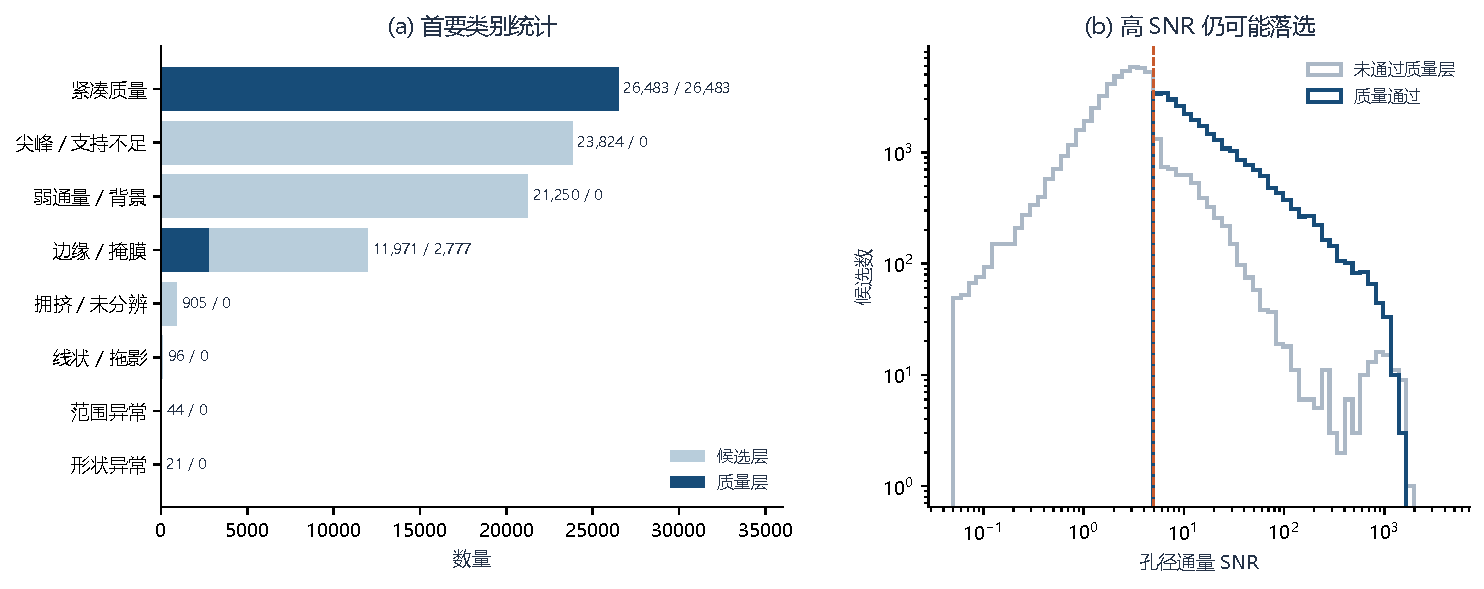
\includegraphics[width=\linewidth]{source_quality.pdf}
\caption{首帧源级统计。左图为首要类别的候选／质量数量，右图为正通量 SNR 的对数分布。未通过质量层的源可以具有很高 SNR；亮度不足不是所有落选源的共同机制。来源为单帧缓存 21。}\label{fig:quality}
\end{figure}

质量通过集合中，2,777 个源的首要类别仍为边缘／掩膜，说明部分有效孔径策略允许其进入质量层。因此“质量通过”等价于当前规则通过，不等价于“没有任何标记”。将完整标记与首要类别同时保留，有利于后续对光度和身份采用更严格的样本选择。

现存缓存的提案计数记录 Gaussian 81,240、窄尺度 DoG 67,815、宽尺度 DoG 60,258，合并后为 84,594。各提案集合高度重叠，上述数量不能相加；也不能由其差额推出每类提案的独立正确率。本文没有在本轮重跑同条件独立检测器对照，因此不将 hybrid 的候选增加量写成精度优势。

\subsection{近邻双响应的原始像素诊断}
源 ID 82931／82934 提供了“多个响应不等于多个独立源”的实例。图\ref{fig:pair} 由首帧原始 FITS 裁剪和缓存质心生成，显示孔径、重复高码和极端负值。已有文档记录整数响应峰距 4.123 px、原图质心距约 2.738 px、半径 4 px 孔径共享 18／49 像素。两者分别具有较高孔径 SNR，但局部测量受到共享亮结构影响。

\begin{figure}[!htbp]\centering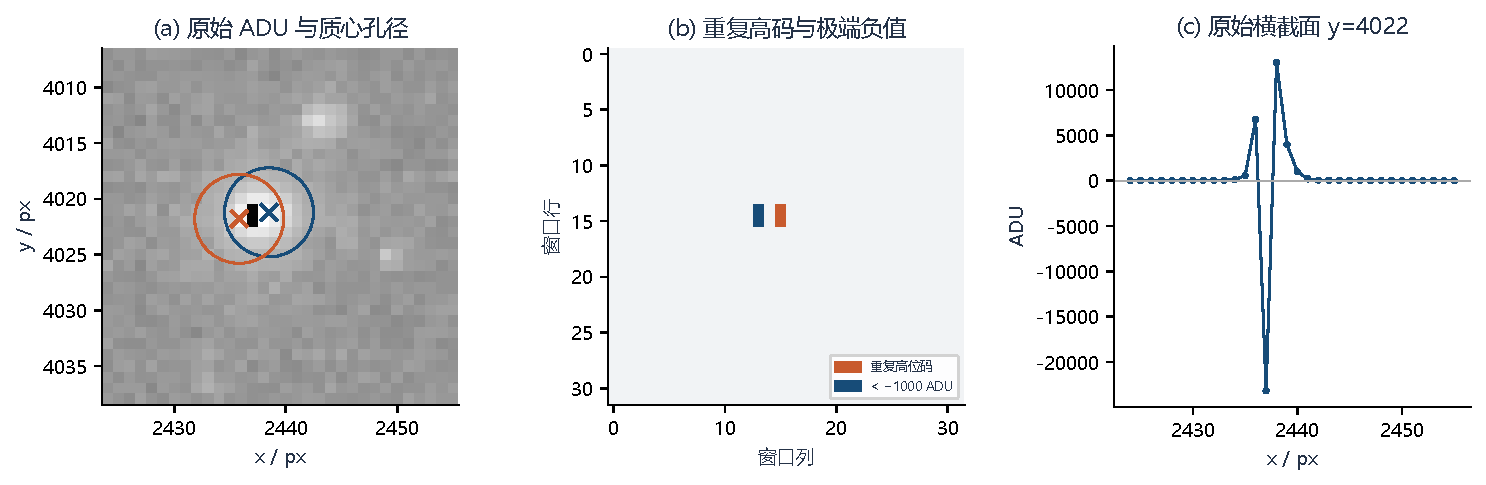
\includegraphics[width=\linewidth]{pair_raw.pdf}
\caption{首帧近邻双响应的原始像素诊断。左图采用对称对数显示以同时呈现强正值与负异常，圆为质心半径 4 px 孔径；中图为局部重复码与极端负值位置；右图为原始 ADU 横截面。显示变换和标记不改变 FITS 数据。}\label{fig:pair}
\end{figure}

历史局部审计记载 raw 双分配为 4／15 帧、双质量为 0／15，屏蔽局部异常值后的双分配下降；自由位置双 PSF 没有稳定通过包含边界条件的确认门。这些属于已有研究记录，本轮未重新运行模型实验。原始裁剪与缓存可直接核对共享孔径和值域结构，已有敏感性记录则支持进一步检查双峰触发机制。

据此，可以拒绝“仅因出现两个框就计为两颗星”的解释，但不能证明该局部完全没有天体信号。优先解释是混合结构经滤波和值域影响形成多个响应；要区分真实混合源与仪器污染，仍需要适用的局部 PSF、独占像素、天空坐标和目录身份。

\subsection{条件化注入回收与质量损失}
已有三布局实验使用首帧真实背景、经验 PSF、2 px 检测尺度和至少 3 个核心支持像素；每条件／强度由三个布局各 8 个无歧义位置组成，共 24 个注入源。经验模板来自 20 个源，记录中位 FWHM 约 2.497 px。表\ref{tab:inject} 和图\ref{fig:inject} 从创新交付审计转录命中数，并重新计算比例与区间。本轮没有找到原布局和注入机读产物，因此将其作为历史实验报告，不宣称重新复现。

\begin{table}[!htbp]\centering\small
\caption{历史三布局实验的候选／质量命中数；每格分母为 24}\label{tab:inject}
\begin{tabular}{l c c c}\toprule
背景条件 & 24 ADU & 56 ADU & 128 ADU\\\midrule
低纹理（blank） & $2/24$；$0/24$ & $22/24$；$1/24$ & $24/24$；$16/24$\\
高背景 & $3/24$；$0/24$ & $21/24$；$2/24$ & $24/24$；$16/24$\\
边缘 & $1/24$；$0/24$ & $19/24$；$0/24$ & $24/24$；$0/24$\\\bottomrule
\end{tabular}
\end{table}

\begin{figure}[!htbp]\centering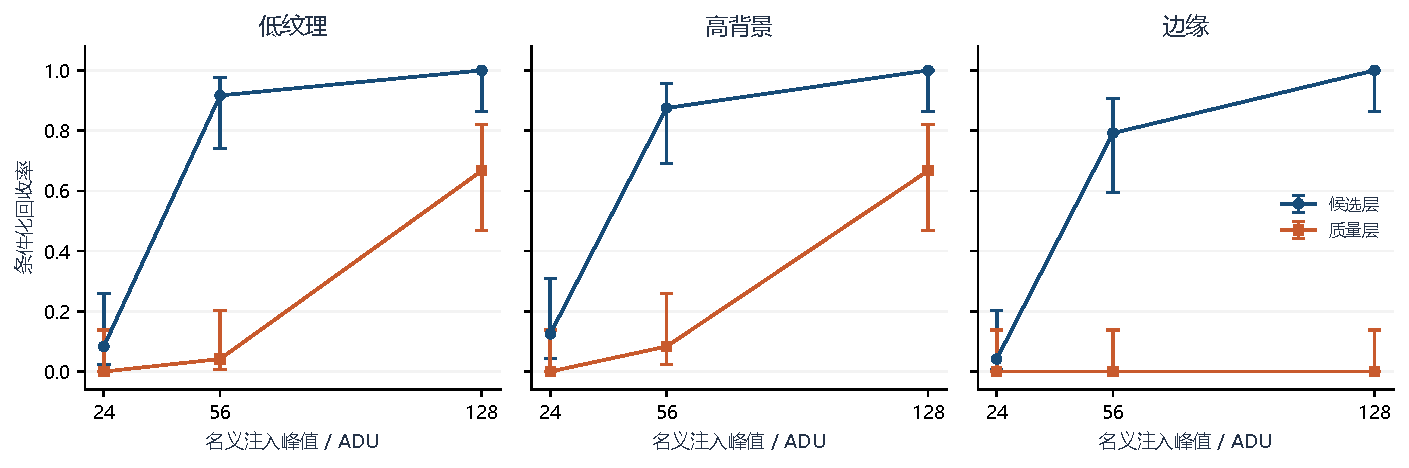
\includegraphics[width=\linewidth]{injection.pdf}
\caption{已有记录的条件化回收率及 Wilson 95\% 描述性区间。每格为三布局共 24 个位置，候选与质量层分别统计。误差条不覆盖共享背景、PSF 失配和布局相关性。}\label{fig:inject}
\end{figure}

128 ADU 时，低纹理和高背景质量回收均为 $66.7\%$，边缘为 0；三种条件候选回收均为 100\%。$24/24$ 的 Wilson 区间约为 $[86.2\%,100\%]$，$16/24$ 约为 $[46.7\%,82.0\%]$，$0/24$ 约为 $[0,13.8\%]$。结果直接说明，边缘条件下“能提出候选”和“满足测量门控”存在显著功能差异；但当前样本和设计不足以声称低纹理与高背景具有显著性能差异。

名义峰值不等于积分通量，也未转换到标准星等。当前实验没有测量全图真实源分布或所有误检，因此不能从这些命中数推出真实全图完备率、precision 或 FDR。若用于正式投稿的核心量化结论，应补回原布局、模板和无注入配对控制，或按相同参数重跑。

\subsection{配准、时序集合与最新缓存结果}
序列缓存 71 的主路径采用平移＋稳健仿射残差，14 个相邻帧启用仿射残差模型，记录配准内点残差中位数 0.1081 px。累计平移最大模长约 0.1772 px，末帧约 $(+0.0410,+0.1322)$ px。图\ref{fig:registration} 显示平移记录和测量工作集质量数；平移曲线不等价于完整仿射模型的误差。

\begin{figure}[!htbp]\centering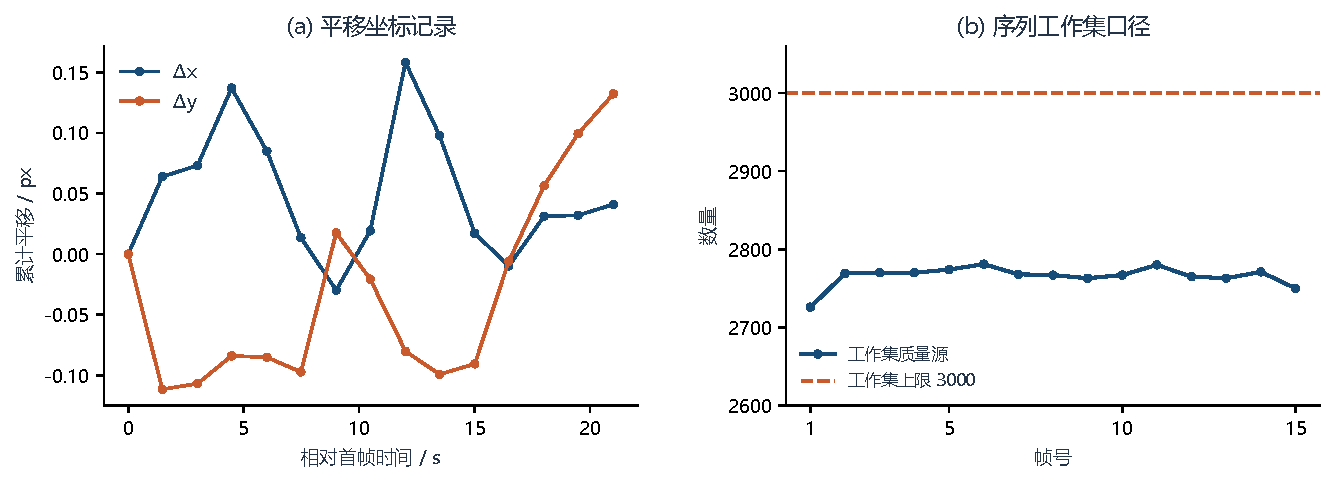
\includegraphics[width=\linewidth]{registration.pdf}
\caption{序列缓存 71 的配准与工作集摘要。每帧全图候选为 83,077--84,653，源级返回固定为 3,000，工作集质量为 2,726--2,781。后两者不代表全图质量源总数。}\label{fig:registration}
\end{figure}

\begin{table}[!htbp]\centering\small
\caption{现存序列轨迹的分类与证据来源}\label{tab:layers}
\begin{tabularx}{\linewidth}{l r Y}\toprule
层级 & 数量 & 语义\\\midrule
严格静态／质量 & 2,334 & 当前质量轨迹的静态分类\\
持续／质量 & 77 & 持续但未入严格静态的质量轨迹\\
瞬态／质量 & 2,290 & 出现不足或未满足持续门的质量轨迹\\
持续／候选共识 & 13,293 & 候选层多帧响应，不是逐帧质量确认\\
持续／时序参考 & 14,507 & 时序参考锚点证据\\
持续／叠加弱源 & 1,468 & 叠加提案回到逐帧窗口得到的证据\\
点源 moving & 0 & 当前点状通道没有通过运动门的轨迹\\
线状 moving／candidate & 4／22 & 当前线状通道的分类结果\\\bottomrule
\end{tabularx}
\end{table}

表\ref{tab:layers} 按现存轨迹列表直接汇总。持续集合包含质量、候选共识和时序参考三个来源；叠加弱源另行输出。不同层级共享图像、模板或预测坐标，不能作为独立证据重复累加。尤其是固定锚点测量可能产生近零位移，这种性质来自测量方式，不构成高精度天体静止的证明。

文档旧稿曾报告严格静态 9,938、持续 6,249 或不同运动数量，其工作集与算法版本不同。本文不将这些数字填入当前参数主表；附录保留差异说明。缓存与当前源码版本字段一致也不等于本轮重新运行了全部算法，本文仅报告产物核对层面的事实。

\subsection{线状运动证据与原图复核}
现存缓存包含四条 \texttt{moving} 线状轨迹，参数和标记见表\ref{tab:motion}。图\ref{fig:motion} 从缓存注册坐标绘制，并使用真实头部时间重新计算 OLS 速度；原缓存的 RMS 保留为算法输出，时间 OLS 的重算值放在交付数据中。

\begin{table}[!htbp]\centering\small
\caption{线状通道当前运动分类；RMS 与 $R$ 为缓存值}\label{tab:motion}
\begin{tabularx}{\linewidth}{l r r r r Y}\toprule
轨迹 & 帧数 & 位移／px & RMS／px & $R$ & 证据与限制\\\midrule
L1 & 15 & 123.504 & 0.344 & 0.899 & 包含预测窗口恢复\\
L2 & 13 & 108.672 & 0.199 & 0.916 & 中心运动与单帧形状\\
L3 & 12 & 114.654 & 0.182 & 0.911 & 非连续观测与单帧片段拼接\\
L4 & 7 & 340.632 & 2.222 & 1.028 & 边缘截断及伪影重叠复核\\\bottomrule
\end{tabularx}
\end{table}

\begin{figure}[!htbp]\centering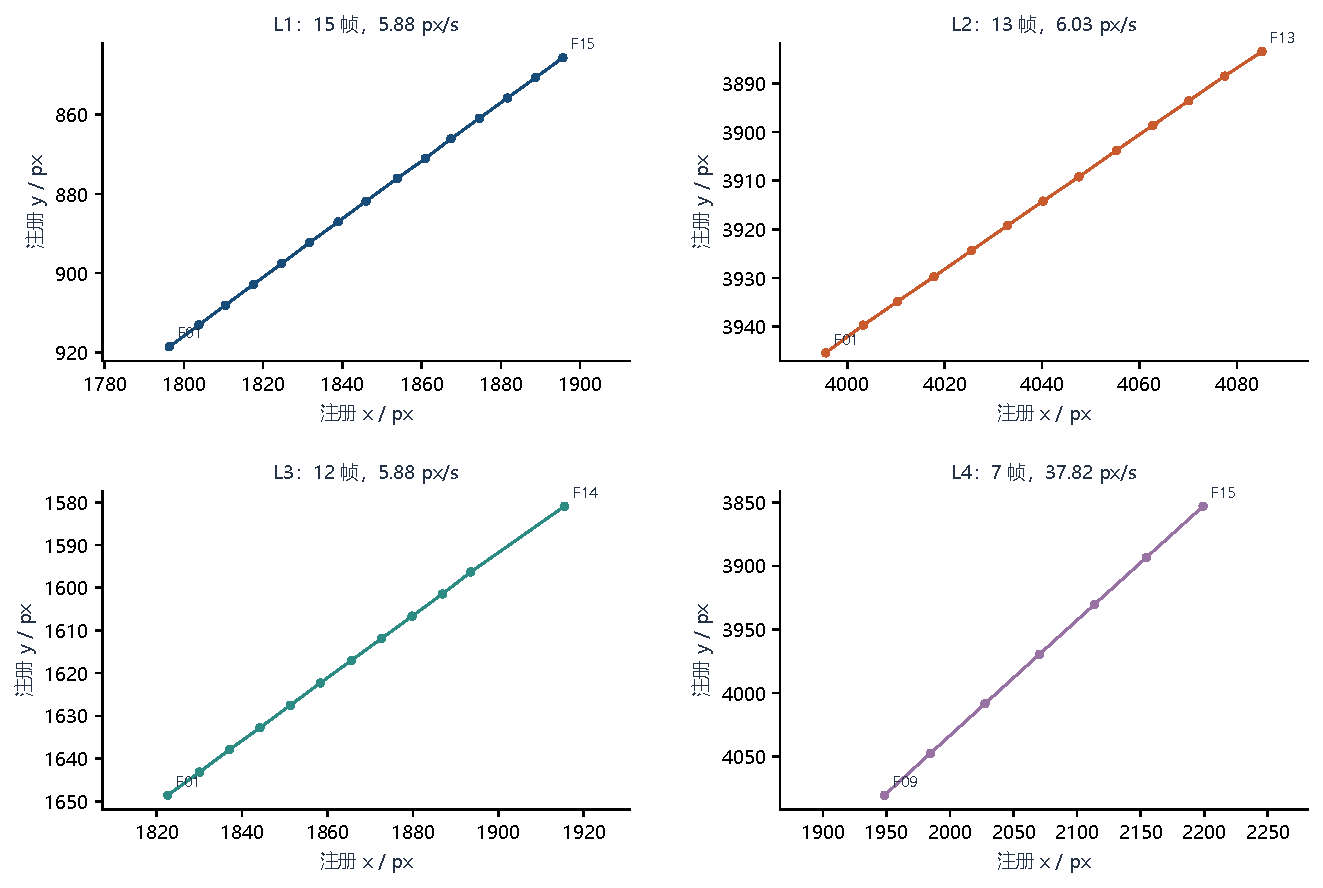
\includegraphics[width=.93\linewidth]{motion_tracks.pdf}
\caption{四条线状缓存轨迹在平移注册坐标中的路径。图中速度由实际 UTC 差和中心坐标重新拟合，单位为 px/s。轨迹编号是当前缓存标识，不表示目标目录身份；预测恢复与仪器冲突需独立审查。}\label{fig:motion}
\end{figure}

L1 涉及预测窗口恢复，因此连续 15 帧中的全部点不能都称作盲检独立命中；L3 的观测帧存在缺口，连续性需依据来源字段复核；L4 保留 \texttt{line\_artifact\_overlap\_reviewed} 证据等级。后者与旧文档中将 F09--F15 保留为冲突候选的口径不同，当前缓存把它归入 moving，但论文仍将该组列为仪器冲突优先复核对象。标签变化并没有消除物理歧义。

图\ref{fig:rawmotion} 对 L1 和 L4 选取四个观测点，在对应原始帧裁剪窗口中展示图像形态。这是数据可视化复核，未增加人工真值标签。单帧长线或持久细线都需要对照背景、固定结构和真实天空映射；其与曝光运动学一致只能提高复核优先级，不能独立证明是某颗卫星或空间碎片。

\begin{figure}[!htbp]\centering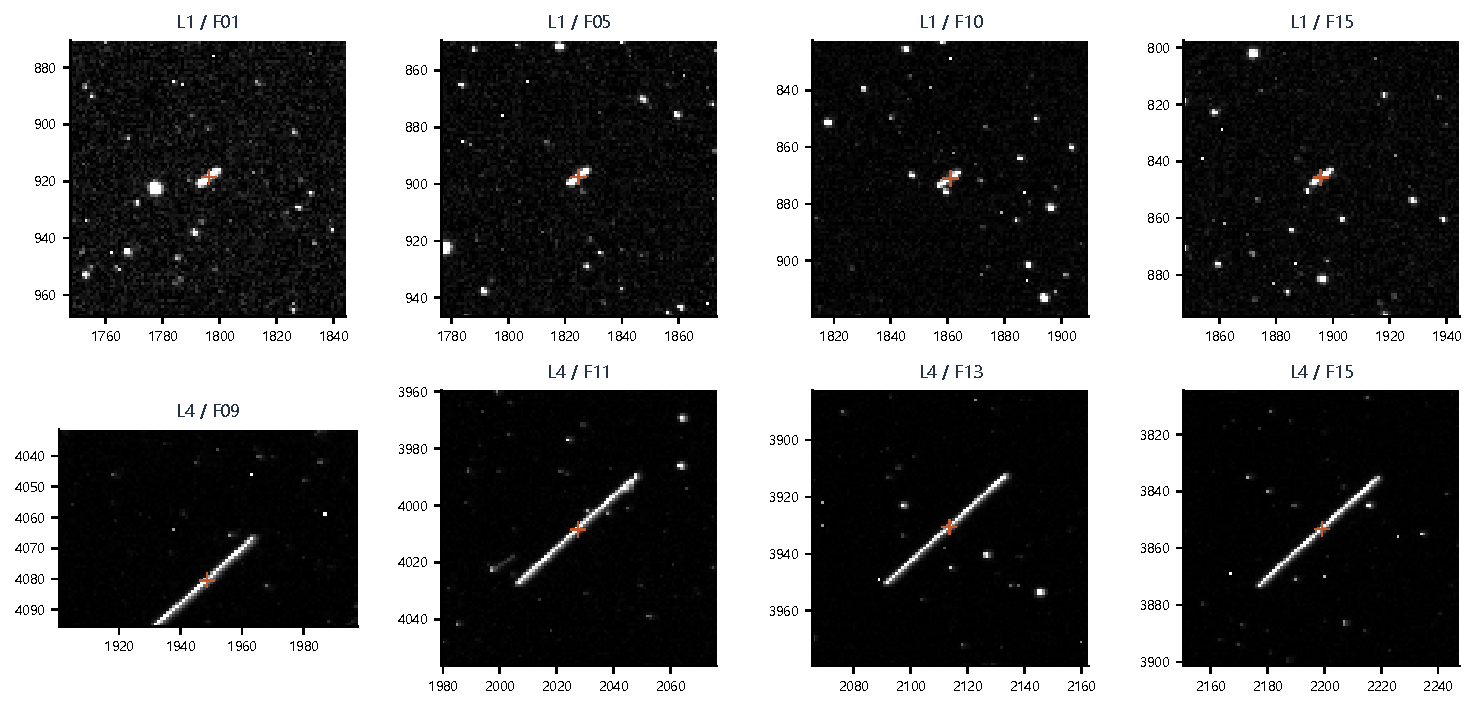
\includegraphics[width=\linewidth]{motion_raw.pdf}
\caption{L1 与 L4 的原始 FITS 时序裁剪。十字为缓存中心，各窗口按自身分位数拉伸以展示形态，灰度不能跨窗口直接比较通量。上行为 L1，下行为带伪影重叠复核标记的 L4。}\label{fig:rawmotion}
\end{figure}

\subsection{最暗质量候选的测光结果}
单帧缓存的 \texttt{faintest\_detected} 为源 80357，坐标约 $(1004.948,3909.962)$ px，净通量 222 ADU，曝光归一通量率为 148 ADU/s，通量 SNR 为 5.0925，仪器星等 $-5.4257$，条件化星等误差约 0.2132 mag。这些值与式\eqref{eq:flux}后的通量率和误差传播关系一致，缓存的标定星等与绝对星等字段均为空。

因此结果可表述为“在当前 29,260 个质量通过源中按仪器通量排序得到的最暗候选”。它不是全图所有物理恒星中已证明最暗的一颗，也不是极限星等；其 SNR 靠近选择门，排序对背景、孔径和光度模型尤其敏感。后续需加入标定后质量门、弱端注入和颜色模型敏感性，才能给出可比较的标准系统结果。

\subsection{注册合成的覆盖与真实性}
现存 NPZ 的位移记录与序列缓存逐项一致，表\ref{tab:mosaic} 汇总核对结果。图\ref{fig:mosaic} 展示 ADU、覆盖与离散度。原图为 $4096\times4096$，输出画布为 $4098\times4098$，但有覆盖面积比为 1.0；新增画布边界没有形成显著新增有效视场。

\begin{table}[!htbp]\centering\small
\caption{现存注册合成数组的元数据}\label{tab:mosaic}
\begin{tabular}{l r}\toprule
指标 & 核对结果\\\midrule
输入／输出尺寸 & $4096\times4096$／$4098\times4098$\\
输入帧数／最大覆盖 & 15／15\\
有覆盖像素 & 16,777,216\\
至少两帧覆盖像素 & 16,777,215\\
有覆盖区平均覆盖 & 14.98876\\
无覆盖像素 & 16,388\\
有效联合面积／单帧面积 & 1.000\\
融合方式／裁剪阈值 & 稳健均值／$3\sigma$\\
最大累计平移 & 约 0.1772 px\\\bottomrule
\end{tabular}
\end{table}

\begin{figure}[!htbp]\centering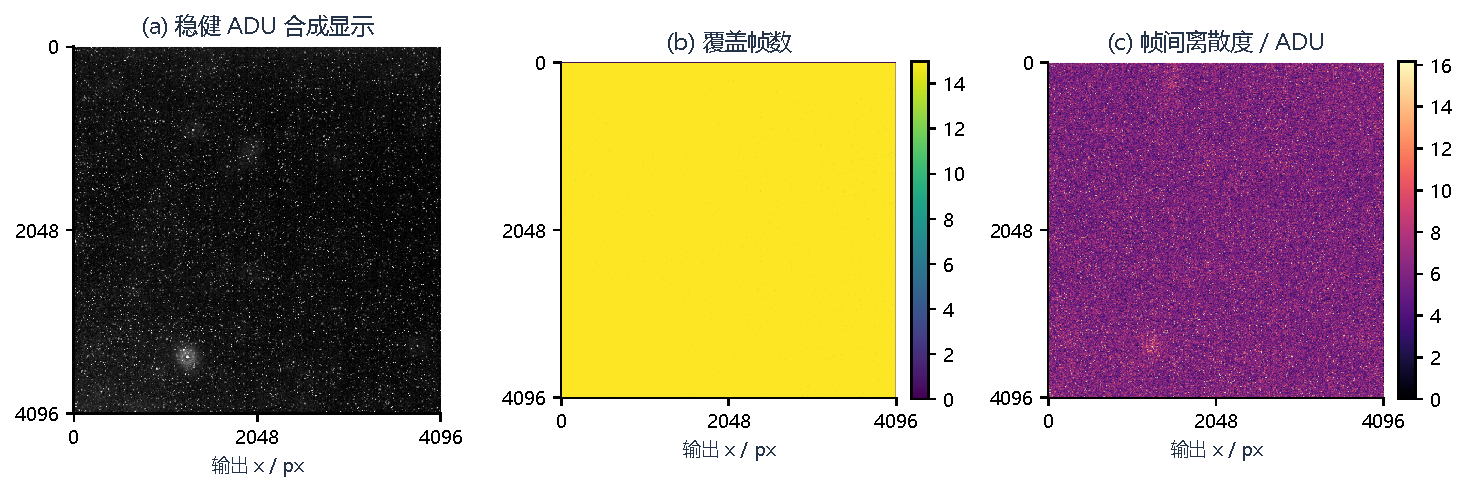
\includegraphics[width=\linewidth]{mosaic.pdf}
\caption{现存平移注册合成的三类图像产品。ADU 图按分位数拉伸，覆盖图保留帧数尺度，离散度图按 99\% 分位截取显示范围。缩略图只用于观察，定量信息由原始 NPZ 保存。}\label{fig:mosaic}
\end{figure}

覆盖数接近 15 表明大多数区域由多帧输入支持，但融合后的噪声不应机械按 $\sqrt{15}$ 改善：重采样、共同背景、相关噪声和稳健裁剪都会改变误差。离散度图可发现时序不一致，却不提供独立恒星身份。此前文档中的约 0.317 px 最大平移属于另一回归记录，本文不与当前 NPZ 的 0.1772 px 混用。

\FloatBarrier
\section{讨论与方法局限}
\subsection{统一系统的价值与证据相关性}
流程的价值在于把异常结构及时交给对应方法，而不是让点检测器承担所有判断。高 SNR 候选可以因为独占像素不足而落选，弱通量候选可以通过多帧参考获得后续复核，线形则进入曝光运动学通道。每一层保留来源，使错误能够定位到提案、测量、关联或身份解释，而非只改变一个总数。

同时，多项指标来自同一像素和检测器，不能被当作彼此独立的验证。原图通量、二维支持和 PSF 相似性共享数据；多帧锚点与配准控制共享源；模型引导的 ROI 恢复使用轨迹预测。将这些证据相乘或简单计票会产生过强置信度。本文采用分层门控与来源标签，不提供未经独立标注训练的恒星概率。

\subsection{统计验证与物理解释的差距}
候选回收回答“已知注入在指定条件下能否被检测”，质量回收回答“同一注入是否满足当前测量规则”。两者都无法单独估计真实源表纯度。符号反相和固定结构阴性对照可以诊断机制，却不能在非对称编码污染下自动等价于真实误检率。对完整性能结论，仍应建立代表性的人工标签、独立星表或可对应的目标真值，并使用空间留出与多布局验证。

测光亦有三层区别：ADU 通量是当前图像量，仪器星等是其对数排序，标准星等依赖零点和波段转换。设备宽谱未知时，简单颜色多项式只能描述经验敏感性，不能代替真实系统响应。最暗端还受检测选择偏差影响，单一最小通量源不应作为设备灵敏度极限。

\subsection{运动候选的误差与身份限制}
图像运动可由真实目标、残余旋转、错误近邻、长线片段或固定结构共同造成。稳健仿射残差能减少群体伪运动，但不能证明所有残差都是天体运动。短轨迹 OLS 误差仅反映所采用模型和中心噪声；它没有包含 PSF 变化、线端截断、系统配准误差和身份歧义。本文不给未经校准的轨道预报区间，也不把四条 moving 等价为四个真实目标。

补充的 16 帧 PIC 测试包与 17 条 POS 记录在目标 ID 和时间上不对应，不能提供逐帧定位误差、precision 或 recall。该材料可以支持配准工程问题的讨论，但不得与主实验 15 帧混合。下一步需要同一目标、同一时间系统、可验证坐标映射的 PIC/POS 配对。

\subsection{可复现性与后续实验}
本文交付的生成脚本从现存缓存重建统计与图件，不改变算法或缓存；输入清单包括文件哈希和时间字段。对缓存核对结果，可复核的是产物身份、内部一致性和原始数据对应关系，不是本次完整运行的性能。历史注入缺少原机读产物，正文已显式标记，正式投稿前应优先补齐这条验证链。

建议后续按以下依赖顺序完善：首先补齐光学响应、增益、噪声、值域和坏像素定义；其次建立全场 WCS 与留出目录残差；再恢复或重跑注入布局与无注入配对控制，扩展空间条件、PSF 和弱端强度；最后建立运动人工真值，评估缺帧恢复、仪器冲突与跨通道去重。参数应由独立验证选择，而不能根据预设星数或目标数调整。

\section{结论}
本文建立了连接点源提案、原图质量测量、测光、多帧关联和图像融合的天基星图分析流程。现存首帧产物核对为 84,594 个候选与 29,260 个质量通过源，类别统计说明落选结构具有多种机制；高 SNR 不足以替代二维支持、值域健康和近邻独立性。已有真实背景实验报告的边缘 $24/24$ 候选命中和 $0/24$ 质量命中，进一步说明发现层与测量层需要分别验证。

现存序列缓存采用每帧 3000 个源的工作集，点状 moving 为 0、线状 moving 为 4。这些是当前门控与证据来源定义下的轨迹结果，其中预测恢复和伪影重叠组仍需专项复核。注册合成同时保留 ADU、coverage 与 scatter，当前有效联合面积未显示显著视场扩大。最暗候选仅有仪器星等，完整光度标定与天体身份尚未闭环。

这些结果支持一套可审计的系统方法，而非物理恒星数或目标识别准确率的最终证明。可靠 WCS、设备标定、独立真值和注入原产物是将工程证据提升到完整科学结论的下一步条件。

\paragraph{作者与声明} 作者：李钧耀；单位：广东科技学院。通信方式及基金信息待补充。原始数据的公开与再分发授权未在当前材料中确认，论文工程不包含原始 FITS。不存在已核验的伦理、利益冲突或数据公开声明，正式投稿时由作者按实际情况填写。

\begingroup\linespread{1.05}\selectfont
\begin{thebibliography}{99}\small
\bibitem{sextractor} Bertin E, Arnouts S. SExtractor: Software for source extraction. Astronomy and Astrophysics Supplement Series, 1996, 117: 393--404. \href{https://aas.aanda.org/articles/aas/pdf/1996/08/ds1060.pdf}{原文链接}.
\bibitem{daophot} Stetson P B. DAOPHOT: A computer program for crowded-field stellar photometry. Publications of the Astronomical Society of the Pacific, 1987, 99: 191--222. \href{https://articles.adsabs.harvard.edu/pdf/1987PASP...99..191S}{原文链接}.
\bibitem{langhogg} Lang D, Hogg D W. Principled point-source detection in collections of astronomical images. 2020, arXiv:2012.15836. \url{https://arxiv.org/abs/2012.15836}.
\bibitem{vio} Vio R, Andreani P. On the correct estimate of the probability of false detection of the matched filter in weak-signal detection problems. Astronomy \& Astrophysics, 2016, 589: A20. \url{https://arxiv.org/abs/1602.02392}.
\bibitem{hedges} Hedges C, Luger R, Martinez Palomera J, et al. Linearized Field Deblending: PSF Photometry for Impatient Astronomers. 2021, arXiv:2106.08411. DOI: \href{https://doi.org/10.3847/1538-3881/ac0825}{10.3847/1538-3881/ac0825}.
\bibitem{astrometry} Lang D, Hogg D W, Mierle K, et al. Astrometry.net: Blind astrometric calibration of arbitrary astronomical images. The Astronomical Journal, 2010, 139: 1782. \url{https://arxiv.org/abs/0910.2233}.
\bibitem{nir} Nir G, Zackay B, Ofek E O. Optimal and Efficient Streak Detection in Astronomical Images. 2018, arXiv:1806.04204. DOI: \href{https://doi.org/10.3847/1538-3881/aaddff}{10.3847/1538-3881/aaddff}.
\bibitem{zogy} Zackay B, Ofek E O, Gal-Yam A. Proper image subtraction: Optimal transient detection, photometry and hypothesis testing. The Astrophysical Journal, 2016, 830: 27. \url{https://arxiv.org/abs/1601.02655}.
\bibitem{fits} FITS Working Group. Definition of the Flexible Image Transport System (FITS), Version 4.0, language-edited edition. 2018（标准于 2016 年通过）. \url{https://fits.gsfc.nasa.gov/fits_standard.html}.
\bibitem{gaia} ESA/Gaia/DPAC. Gaia DR3 passbands. \url{https://www.cosmos.esa.int/web/gaia/dr3-passbands}. 访问日期：2026-10-10.
\bibitem{comest} Chiu I-N, Desai S, Liu J. ComEst: A Completeness Estimator of Source Extraction on Astronomical Imaging. 2016, arXiv:1605.02650. DOI: \href{https://doi.org/10.1016/j.ascom.2016.04.005}{10.1016/j.ascom.2016.04.005}.
\end{thebibliography}
\endgroup

\clearpage\appendix
\section{证据索引与复核范围}
本附录将本次核对和历史记录分开。原始数据与缓存没有随论文工程打包；交付的输入清单、证据摘要和来源说明记录身份与核查范围。表\ref{tab:evidence} 为简要索引，完整哈希保存在外部清单，避免长路径挤占正文。

\begin{table}[!htbp]\centering\small
\caption{结果来源与本次验证层级}\label{tab:evidence}
\begin{tabularx}{\linewidth}{l Y Y}\toprule
结果 & 来源 & 本次核对范围\\\midrule
15 帧格式与时间 & 原始 FITS、序列输入身份 & 文件 SHA-256、头部与尺寸\\
首帧 84,594／29,260 & 单帧缓存 21 & 记录数、质量和类别汇总\\
最暗仪器候选 & 同一单帧缓存 & 通量率、仪器星等与状态\\
序列静态／运动 & 序列缓存 71 & 工作集、轨迹来源、坐标与时间\\
四条线状路径 & 同一序列缓存 & 原图裁剪、时间 OLS 重算\\
注册合成 & 现存 mosaic NPZ & 数组、元数据与位移一致性\\
三布局注入 & 创新交付审计 & 文档转录、比例与区间重算\\
双响应敏感性 & 核心短稿与研究记录 & 原图裁剪；未重跑模型实验\\\bottomrule
\end{tabularx}
\end{table}

单帧缓存文件哈希、序列缓存文件哈希和 NPZ 文件哈希由生成脚本计算；原始 FITS 每个输入也重新核对。哈希能证明本次引用的字节身份，不能证明算法正确或物理真值。当前工作区存在已有修改，论文交付不修改这些文件，也没有对现有算法做新测试或完整运行。

\subsection{旧稿与主结果差异}
旧核心短稿记录点源 moving 为 0、连续线状 1 条加单帧候选 1 条；更新的关系说明另记录 4 点状、2 线状及跨通道去重。现存序列缓存 71 则为点状 0、线状 4、22 条线状 candidate，来源字段进一步包括预测恢复和伪影重叠复核。本文主结果使用当前可核对缓存，并在正文保留其中的适用域限制，未将旧稿混成同次实验。

旧合成文档的最大累计平移约 0.317 px，与现存 NPZ 约 0.1772 px 不同；两者的输出尺寸相同并不能证明参数相同。现存 NPZ 与当前缓存的累计位移逐项一致，所以正文采用现存数组。历史 9,938 严格静态和 6,249 持续候选亦不进入当前 3000 工作集主表。

\subsection{历史实验的引用位置}
三布局注入命中数来自 \texttt{doc/04-创新分析/创新交付审计.md} 中“当前主结果：三布局核心条件实验”，该记录指定首帧、三个条件、三个名义强度和每格 24 个源。双响应敏感性来自 \texttt{doc/05-论文答辩/竞赛论文核心短稿.md} 的近邻案例及相关来源账本。它们是项目内部数据记录，不作为外部已发表研究引用；其机器输出缺失对可复现性的限制已经说明。

\section{区间、误差与复现补充}
\subsection{Wilson 描述性区间}
对 $k$ 次命中、$n$ 个已知注入，令 $\widehat p=k/n$、$z=1.95996$，区间中心和半宽为
\begin{align}
 c&=\frac{\widehat p+z^2/(2n)}{1+z^2/n},\\
 w&=\frac{z}{1+z^2/n}\sqrt{\frac{\widehat p(1-\widehat p)}{n}+\frac{z^2}{4n^2}}.
\end{align}
报告 $[c-w,c+w]$。这一计数区间用于展示小分母带来的不确定性，不能覆盖同一布局的空间相关、背景复用、模板偏差或位置选择。由名义强度到物理灵敏度还需要标准测光与完整选择函数。

\subsection{坐标、速度与恢复点}
原图坐标以左上为原点、x 向右、y 向下；原始帧号在内部以零开始，论文图表统一以 F01--F15 展示。图像方向与赤经赤纬方向不同。时间 OLS 使用每个实际观测点的 UTC 差，保留缺帧而不按均匀帧距补齐。缓存字段 \texttt{speed\_px\_per\_frame} 不用于本文速度主图，避免将历史兼容字段直接解释为真实时间速度。

预测 ROI 恢复点的数量与来源保存在 \texttt{motion\_cache.csv}。它们可用于检验轨迹持续性，但应与原始检测点分开评价恢复率。若评估运动目标性能，需要预先确定匹配容差、独立真值和逐帧漏检定义，不能在轨迹拟合后选择有利的判定规则。

\subsection{补充 PIC/POS 数据的配对障碍}
2026-09-13 的定位数据 checkpoint 记录 PIC 含 16 帧、时间为 2026-06-15 15:30:36.5380--15:31:30.7010 UTC；POS 含 17 行、时间为 15:38:08.9850--15:39:00.1400 UTC。包名目标 ID 分别为 39155 与 44299，辅助字段在该 PIC 数据中全零。没有可靠时间和目标对应关系时，两包仅能用于图像处理与格式测试，不能提供逐帧定位误差真值。

\subsection{复现工程与待补输入}
交付工程使用 XeLaTeX，正文与参考文献在 \texttt{main.tex}，图表由 \texttt{prepare\_assets.py} 从本地现存产物生成。已打包图件可直接用于论文编译；重建数据图件需要原始 FITS 与相应缓存。\texttt{build.ps1} 将编译中间文件放入 \texttt{tmp}，最终 PDF 放入 \texttt{output/pdf}。

完整算法复现还需补充与缓存对应的源码快照、解析后的全部参数、设备误差输入及历史注入机读输出。投稿前需由作者补充通信方式、基金、目标期刊声明和数据可用性说明，并补齐 WCS、标定与真值验证。本文已将这些未知条件保留为限制，不填入虚构数据。
\end{document}
